\documentclass{article}
\usepackage[utf8]{inputenc}
\usepackage[margin=0.6in]{geometry}
\title{\bf { Some positive thoughts about Negative Absolute Temperature}}
\author{Anuradha $\text{Gupta}^{1}$ and Deepak $\text{Jain}^2$ \\
\\
(1) S.G.T.B. Khalsa College\\
University of Delhi\\
Delhi 110007, India\\
\\
(2) Deen Dayal Upadhyaya College\\
(University of Delhi)\\
Sector-3, Dwarka,\\
New Delhi 110078, India\\
\\
email: anuradha@sgtbkhalsa.du.ac.in\\
djain@ddu.du.ac.in}
\date{}
\usepackage{amsmath}
% \usepackage[square,sort,comma,numbers]{natbib}

% \usepackage{natbib}
\usepackage{graphicx}
\begin{document}
\large
\maketitle
\begin{abstract}
\large  It is now widely accepted that the concept of negative absolute temperature is real one  and not just theoretical curiosity.
In this brief report, by  combining the  formalism used in the statistical mechanics and thermodynamics,  we have explained   some aspects of  negative temperature ( both mathematically and graphically ) in the two level system. We believe that these simple  calculations may give  useful and concrete insights  about the negative absolute temperature to the undergraduate students.
\end{abstract}

\maketitle

\section{Introduction}
Traditionally the temperature of  an ideal gas, consisting of point mass particles,  is explained by establishing its relation with  average kinetic energy. For a crystalline solid, the temperature is connected to the  vibratory motion of nuclei about their mean positions. These connections have opened up a door to link the thermodynamic properties  to a microscopic  atomic structure. Further important insight of microscopic world can be obtained by  Boltzmann definition of entropy.  This established an association  of  the observable quantities of the macroscopic world ( Thermodynamics) with the microscopic one ( Statistical mechanics) through a relation $$ S = \, k_B\, ln  \, \Omega $$
Here entropy, S, is a macroscopic parameter written in term of microscopic quantity called multiplicity of a state ( $ \Omega$) and $k_B$ is the Boltzmann constant. 
 In thermal physics,  the concept of temperature is introduced as the relationship between the entropy (S) and the internal energy (U). 

$$ {1 \over T} = {\left( {\partial S \over \partial U }\right)_{V,N}}
$$
Where N and V are number of particles and volume respectively.
Hence by using the above  definition, the temperature  can be rewritten as 
$$ {1\over T} = \, {  k_B} {\left(  \partial ln \, \Omega \over \partial U \right)_{V,N}}
$$

 {\it The temperature remains positive} if entropy is an increasing function of internal energy i.e gas consisting of free particles. In this type of physical system there is a lower bound on the energy  and the lower level is more populated than the upper level.This can be understood from the fact that occupation number of each level is proportional  to the Boltzmann factor 
 $$ N_i\, \propto \, e^{-\epsilon_i / k_BT} $$
 So  the normalization factor for these $N_i$ , popularly known as partition funtion,  converges only if there is a lower bound on the $\epsilon_i$  for positive temperature state.
There exists another class of physical systems  where the entropy decreases with the increase in the internal energy {\it hence the temperature becomes negative}.  In this type of system, there is a finite upper bound to the energy spectrum and the higher energy state are more populated than the lower energy state again to facilitate the convergence of partition function.
This concept of negative absolute  temperature is known since the work done by Onsager on 
vortices  present in the 2-dim.  hydrodynamics{\cite{1}}. But experimentally the negative temperature  was first observed in magnetic  nuclear spin system by Purcell and Pound in the year 1951{\cite{2}}.  Recently it has been achieved in the ultra cold bosons in the optical lattices{\cite{3}}. For the complete history of negative temperature and its implications on the thermodynamics,  controversies and recent developments etc. ,  see the following ref's {\cite{4,5,6,7,8,9,10,11,12}}.
 \vskip 0.4 cm
 \noindent  Motivated by the previous work in the literature about the negative temperature, in this paper
  we elaborate two important issues related to negative temperature.
First, evaluate the entropy and internal energy of a finite level system when the   population  of the  energy levels changes( we consider two levels in this work). The idea is to check what would happen to the temperature of such a system with the  gradual change in the number of particles of the two levels. The second objective is to obtain the general expression of S (entropy) in terms of  U ( internal energy) and N ( number of particles) by using the Lagrange interpolation method. We also believe that the above mentioned points related to the negative temperature have not been addressed adequately in the literature. \vskip 0.3 cm
 \noindent The outline of the paper is as follows: In section 2, we describe the set of equations for calculating the entropy of a  two level system in various configurations of particle distributions. The Lagrange interpolation method along with its application to  finite level system is presented in section 3. Finally, the results are discussed in section 4. 
 
\vskip 0.4 cm
\section{ Entropy, S(U),  of a finite level system}

In this section we obtain the expressions of entropy and internal energy at various configurations of  states defined by the distribution of particles in the two level system. We start with first case A; when the lower level of energy $\epsilon_1$ is fully populated with $ N_1 = N$ particles and upper level of  energy $\epsilon_2$ is completely vacant, $N_2 = 0$. Subsequently, we obtain both S and U for different cases when the population of lower level keep on decreasing and occupancy of high level goes on increasing. In other words we start with the case when $ N_1 = N$ and $ N_2 = 0$ and cover the  entire range of variation of particles till $ N_1 = 0$ and $ N_2 = N$. The variation of entropy w.r.t. internal energy is plotted in Figure 1 and corresponding various configuration of particles in  two levels are plotted in the Figure 2. Furthermore, a glance on Figure 1 shows that it is symmetric about the point $U_D$ which corresponds to the maximum entropy of the given system. In this work we have assumed two level system with energy  $ \epsilon_1 \, < \, \epsilon_2$ and $ N_1 + N_2 = N$. 
The details of calculations of $S$ and $U$ for various distribution of particles are as follows:
\begin{figure}[ht!]
\centering
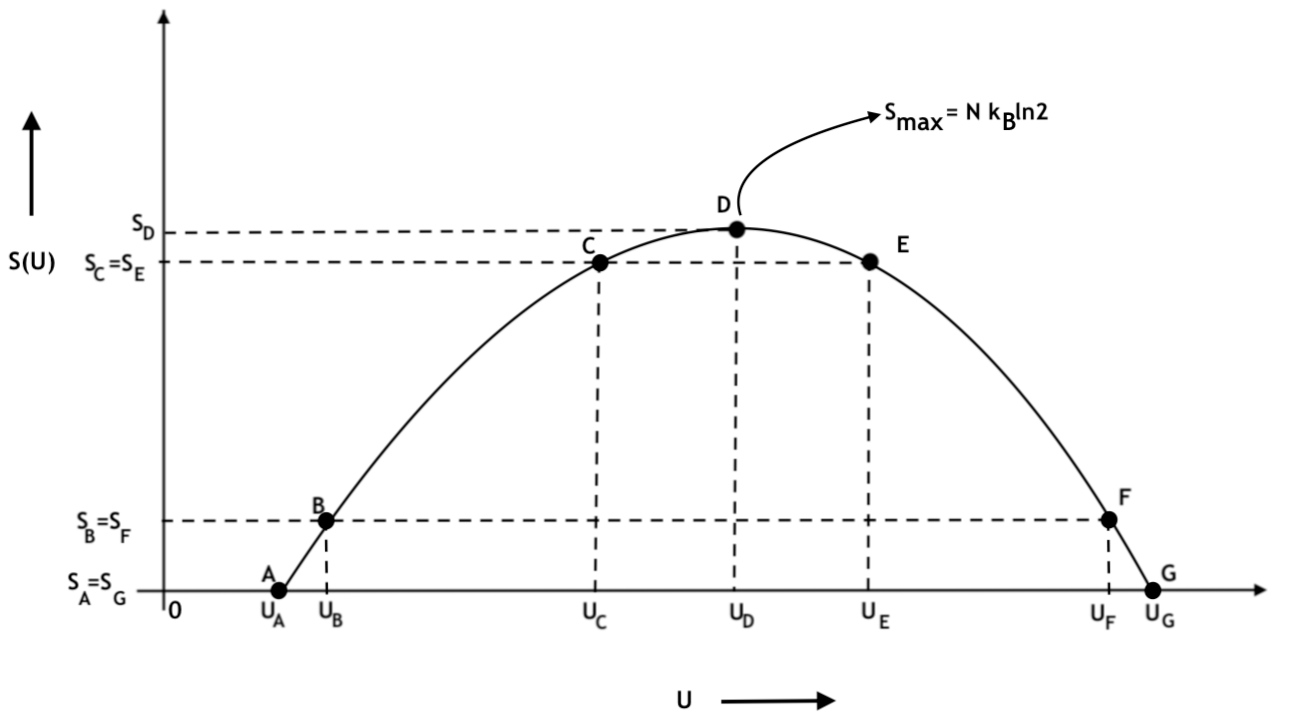
\includegraphics[scale=0.4]{1A.png}
\caption{ S versus U in a two level system}
\label{6}
\end{figure}

\begin{figure}[ht!]
\centering
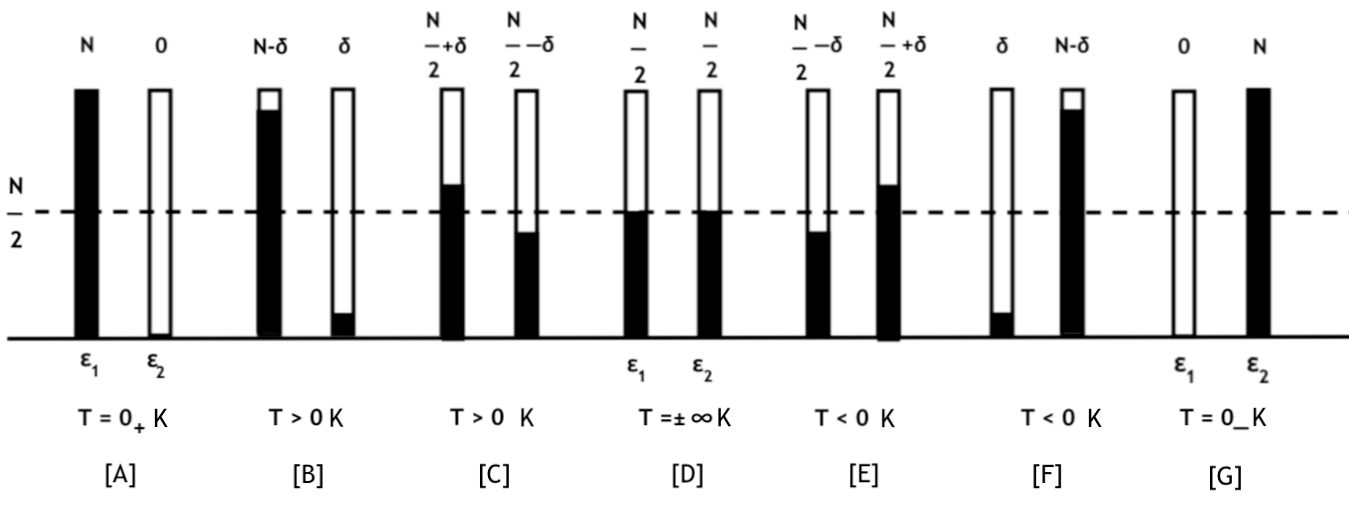
\includegraphics[scale=0.4]{2A.png}
\caption{Distribution of particles in a two level system where $\epsilon_1 \, < \, \epsilon_2$}
%\label{6}
\end{figure}
\vskip 1 cm
{\bf Case A: Minimum entropy}
\vskip 0.3 cm
$ N_1  = N $ and $N_2 = 0$ , Internal energy  is $ U_A = N\epsilon_1$
\vskip  0.4 cm
The entropy at point A can be expressed as:
$$ S_A = k_B \, ln \, \Omega  = \,\,k_B\,\, ln \,{ N! \over {N_1! \, N_2!}} =\,k_B\, ln \,{ N! \over {N! \, 0!}}= k_B\, ln \,(1)\, = \, 0$$  
\vskip 0.5cm

{\bf Case B: Evaluation of S and U at a point close to minimum entropy configuration}
\vskip 0.3 cm
 $N_1 = {N} - \delta $ and $N_2 = \delta $, 
 \vskip 0.3 cm
 Internal energy , $U_B = ({N} - \delta)\epsilon_1 + (\delta)\epsilon_2 = {N} \, \epsilon_1  \, + \,  \delta ( \epsilon_2 - \epsilon_1)$
 \vskip 0.3 cm
 The entropy at point B is equal to : 
 $$ S_B= \, k_B \, ln \,\,{ N! \over { ( {N} - \delta )!\, (\delta )!}} = k_B\,\left[ \, N\, ln \,N - \, N - \,( {N} - \delta )\, ln\, ( {N } -  \delta ) + ( {N } - \delta )\, \right]$$
 
 Since $\delta < < N$, so $ln \, \delta !$ is negligible compare to $ln \,(N - \delta) !$ and $ln \, N !$.

On solving the above equation , we get :

$$ S_B \, = \, k_B\, \left[ \, \delta\, ln \, N - { \delta^2 \over {2 N}}\right]\, = \,  k_B\, \delta\, ln \, N - { k_B\,\delta^2 \over {2 N}}$$

\vskip 0.5 cm
{\bf Case C: Evaluation of S and U  at a point close to maximum entropy configuration}
\vskip 0.3 cm
 $N_1 = {N \over2} + \delta $ and $N_2 = {N \over2} - \delta $, 
 \vskip 0.3 cm
 Internal energy , $U_C = ({N \over2} + \delta)\epsilon_1 + ({N \over 2} -\, \delta)\epsilon_2 = {N\over 2} \,( \epsilon_1 + \epsilon_2) \, + \,  \delta ( \epsilon_1 - \epsilon_2)$
 \vskip 0.5 cm
 The entropy at point C is equal to : 
 $$ S_B= \, k_B \, ln \,\,{ N! \over { ( {N \over 2} +  \delta )! ( {N \over 2} -  \delta )!}} = k_B\,\left[ \, N\, ln N - \,( {N \over 2} +  \delta )\, ln\, ( {N \over 2} +  \delta ) - ( {N \over 2} - \delta )\, ln \,( {N \over 2} -  \delta )\right]$$
 
 Using the approximation $ \delta \, << \, { N \over 2}$, we get:
 $$ S_C \, = \, k_B \left[ N \, ln \, N \,  - N \, ln { N \over 2} - {2 {\delta^{2} \over N} } \right ] = \, k_B \, ln\, {2^N}\, - {2\, k_B\, {\delta^{2} \over N} }$$
 
 \vskip 0.5 cm
 
{\bf Case D: Maximum entropy configuration}
\vskip 0.3 cm
$N_1 = { N \over2}$ and $N_2 = { N \over2}$
\vskip 0.3 cm
Internal Energy, $U_D = {N \over2} \, ( \epsilon_1 \, + \epsilon_2)$
\vskip 0.3 cm
Entropy at D: 
$ S_D =\,  S_{max} = \, k_B \, ln\, {2^N}$

\vskip 0.5 cm

{\bf Case E:  Evaluation of S and U at a point close to maximum entropy configuration}
\vskip 0.3 cm
 $N_1 = {N \over2} - \delta $ and $N_2 = {N \over2} + \delta $, 
 \vskip 0.3 cm
 Internal energy , $U_E = ({N \over2} - \delta)\epsilon_1 + ({N \over 2} +\, \delta)\epsilon_2 = {N\over 2} \,( \epsilon_1 + \epsilon_2) \, + \,  \delta ( \epsilon_2 - \epsilon_1)$
 \vskip 0.3 cm
 The entropy at point E is equal to : 
 $$ S_E \,= \, k_B \, ln \,\,{ N! \over { ( {N \over 2} -  \delta )! ( {N \over 2} + \delta )!}} = k_B\,\left[ \, N\, ln N - \,( {N \over 2} +  \delta )\, ln\, ( {N \over 2} +  \delta ) - ( {N \over 2} - \delta )\, ln \,( {N \over 2} -  \delta )\right]$$
 
 Using the approximation $ \delta \, << \, { N \over 2}$, we get:
 $$ S_E \, = \, k_B \left[ N \, ln \, N \,  - N \, ln { N \over 2} - {2 {\delta^{2} \over N} } \right ] = \, k_B \, ln\, {2^N}\, - {2\, k_B\, {\delta^{2} \over N} } = \, S_C$$
 
\vskip 0.5 cm

{\bf Case F: Evaluation of S and U at a point close to minimum entropy configuration}
\vskip 0.3 cm
 $N_1 = \delta $ and $N_2 =  N - \,\delta $, 
 \vskip 0.3 cm
 Internal energy , $U_F = {N}\epsilon_2  -\,  \delta ( \epsilon_2 - \epsilon_1)$
 \vskip 0.3 cm
 The entropy at point F is equal to : 
 $$ S_F= \, k_B \, ln \,\,{ N! \over {(\delta )! \,( {N} - \delta )! }} = k_B\,\left[ \, N\, ln \,N - \, N - \,( {N} - \delta )\, ln\, ( {N } -  \delta ) + ( {N } - \delta )\, \right] $$

On solving the above equation , we get :

$$ S_F \, = \, k_B\, \left[ \, \delta\, ln \, N - { \delta^2 \over {2 N}}\right] \, = \, S_B$$
\vskip 0.5 cm

{\bf Case G:  Minimum entropy}
\vskip 0.3 cm

$ N_1  = 0 $ and $N_2 = N$ , Internal energy  is $ U_G = N\epsilon_2$
\vskip  0.4 cm
The entropy at point G can be expressed as:
$$ S_G = k_B \, ln \, \Omega  = \,\,k_B\,\,ln\, { N! \over {N_1! \, N_2!}} = k_B\, ln (1)\, = \, 0  =\, S_A$$  
\vskip 0.5cm
The results obtained above are mentioned in the Table {\ref{1T}}. One can clearly observe that as we move from point $A$ to $D$, the entropy increases from zero to its maximum value at point $D$ and after that it decreases continuously  as we move from  $D$ to the point $G$. On the other hand, the internal energy $U$, keeps on increasing continuously from Point $A$ to $G$. 

Another interesting feature of this calculation  is the change in the magnitude of the entropy of the system with the variation of number of particles occupying the two levels of the system. In the vicinity of the minimum entropy position ( point A or G), the change in the entropy  is maximum when we move from $A$ to point $B$  ( assume $\delta = 1$) or from $ F$ to $ G$.
Similarly the change in entropy is minimum  in the vicinity of maximum entropy position. ( For example when move from point $C$ to $D$ or from $D$ to $E$ and assume $\delta = 1$). Hence the variation of entropy is steep  with the change in the number of particles close to the minimum  position. Furthermore the   variation of $S$  slows down and becomes almost flat at the maximum position. This behaviour of entropy is symmetrical and hence one can easily co-relate this variation with the inverted parabola graph.
 
\begin{table}[ht]
\centering
\renewcommand{\arraystretch}{3}
\begin{tabular}[b]{| c | c| c| c| c|}\hline
 Case & $N_1$ & $N_2 $& Internal Energy (U) & Entropy (S) \\ \hline \hline
A & N & 0 &$ N\,\epsilon_1 $& 0\\ \hline
B & $N - \, \delta$& $\delta$ & $ {N} \, \epsilon_1  \, + \,  \delta ( \epsilon_2 - \epsilon_1)$& $ k_B \, \delta\, ln \, N - \, k_B{\delta^2 \over {2 N}}$\\ \hline
C & ${N/2} + \, \delta$&${N/2} - \, \delta$& ${N\over 2} \,( \epsilon_1 + \epsilon_2) \, - \,  \delta ( \epsilon_2 - \epsilon_1)$ & $ k_B \, ln\, {2^N}\, - {2\, k_B\, {\delta^{2} \over N}} $\\ \hline
D & N/2 & N/2 & ${N\over 2} \,( \epsilon_1 + \epsilon_2)$ & $ k_B \,ln\, 2^N$\\ \hline
E & ${ N / 2 } - \, \delta$ & ${N/2} + \, \delta$ & ${N\over 2} \,( \epsilon_1 + \epsilon_2) \, + \,  \delta ( \epsilon_2 - \epsilon_1)$ & $ k_B \, ln\, {2^N}\, - {2\, k_B\, {\delta^{2} \over N}}  $\\ \hline
F & $\delta$ & $N -\, \delta$ & $ {N} \, \epsilon_2  \, - \,  \delta ( \epsilon_2 - \epsilon_1)$&  $ k_B \, \delta\, ln \, N - k_B\,{ \delta^2 \over {2 N}}$\\ \hline
G & 0 & N & $ N \, \epsilon_2$ & 0\\ \hline
\end{tabular}
\caption{ Brief summary of the parameters obtained in the two level system}
\label{1T}
`\end{table}

\vskip 0.5cm
\section{ General expression of \,\,S(U, N)}

In the previous section we obtained the values of entropy for a two level system  for various distribution of particles in it.  In this section we will focus on the construction of a smooth polynomial\,  (Here S(U))  by using the data  obtained in the form of  $( S_i, U_i)$ in the previous section.
We use Lagrange interpolation method      to find the general form of entropy  as a function of  internal energy. In this method the $n^{th}$ order polynomial is constructed by using $n+1$ data points. 
This can be further written as 
$$ S_{ip}(U) = \, \sum_{i = 1}^{ n} L(U_i)S_i  = L( U_1)\,S_1 + L(U_2)\, S_2 + \, L(U_3) \, S_3 + ..... +\, L(U_n) \, S_n $$ 
\vskip 0.3 cm
\noindent Here $S_{ip}$ is known as interpolating polynomial of degree $n$. The  points $U_1, U_2, ....U_n$ are interpolation points and $L(U)$  is known as Lagrange polynomial. As mentioned in the previous section,  the graph between $S$ and $U$ is an inverted parabola so we assume $S$ to be a second order polynomial and hence use the three data points. This  parabolic variation between $S$ and $U$ is also supported by Masthay and Fannin {\cite{13}}. The three data points used to obtain the general form of $S$ are $(U_A, S_A)$,$(U_C, S_C)$ and  $(U_G, S_G)$ at the points $A$, $C$ and $G$ respectively {\footnote{one can also obtain the general form of S(U) by assuming any three points as shown in Figure 1.}}.
For more details of this method see {\cite{14}}.

\vskip 0.4 cm
\noindent Now the general form of $ S_{ip}(U,N)$ in this case becomes:
\begin{equation}
S_{ip}(U, N)  = L(U_A) S_A + L(U_C) S_C + L(U_G) S_G
\label{a}
\end{equation}
\vskip 0.3 cm
as both $ S_A = S_G = 0$, hence $ S_{ip}(U)  = L(U_C) S_C $
\vskip 0.4cm
By definition, the basis polynomial, $L(U_C)$ is written as:

$$ L(U_C) =\, {{(U - U_A) (U - \, U_G)}\over{(U_C - \, U_A) ( U_C - \, U_G)}}$$

After substituting the values of $U_A,\, U_C, \, U_G$ and $S_C$  in the eq.{\ref{a}}, we finally get:

$$S_{ip}(U, N) \,= S_C \, \left[ {( U - N\epsilon_1) \, ( U - N\epsilon_2) }\over { ( { N \over 2} (\epsilon_1 + \epsilon_2) + \delta (\epsilon_1 - \epsilon_2) - \, N \epsilon_1) \left( { N \over 2} (\epsilon_1 + \epsilon_2) + \delta (\epsilon_1 - \epsilon_2) - \, N \epsilon_2 \right)} \right]$$
\vskip 0.5 cm

\begin{equation}
 \boxed{S_{ip}(U, N)\,=  \left[  \,k_B \, ln \,2^N\, - { 2\,k_B\, \delta^2 \over N} \right]\left[ U^2 \, - { N (\epsilon_1 + \epsilon_2) U \, + N^2 \epsilon_1 \epsilon_2 }\over { ( \delta^2 - { N^2 \over 4} ) (\epsilon_1 -\epsilon_2)^2 } \right]}
 \label{b}
\end{equation}

\vskip 0.5 cm


\noindent One can easily check that the above expression ( eq.{\ref{b}}) reduces to the entropy at point $D$ ( $S =\, S_D =  N\, k_B\, ln2)$ in the limit $\delta \rightarrow 0 $. Similarly as expected, we can also recover the entropy at point $A$ , $C$ and $G$ with the general expression of entropy.
We further checked the eq.{\ref{b}}  for the  two level magnetic system  in which each spin dipole has  energy levels $ \epsilon_1 = \, - \epsilon$ and $ \epsilon_2 = \epsilon$. The entropy for such a system can  be written as:
\begin{equation}
 S(U, N)\,=  \,\left[ k_B \, ln \,2^N\, - { 2\,k_B\, \delta^2 \over N} \right] \left[ {  1 \,-{ U^2 \over {N^2\epsilon^2}} } \right]
 \left [{ { 1 -\, {4\delta^2 \over N^2} }} \right]^{-1}
 \end{equation}

\section{Discussion}
We investigated two issues related to the negative absolute temperature which have not been highlighted explicitly in the literature. Hence
the importance of this study is twofold: 
\vskip 0.5 cm
\noindent {\bf First}, We show  the behaviour of entropy close to the maxima point when population in both the levels is equal. Similarly the values of entropy are obtained close to the minima point when one of the level is fully occupied while the other one is vacant.  It clearly indicates that the graph between entropy and internal energy is symmetrical in nature. The internal energy increases continuously from the point $A$ to $G$ while entropy increases only from the point $A$ to $D$  and hence we obtain positive temperature in this region. While as we move from $D$ to $G$, the entropy starts decreasing ( see Fig.1)  but internal energy is still increasing , hence the temperature becomes negative in this right half of the graph.  The concept of positive and  negative absolute temperature can be understood from the Figure 1 by invoking  Boltzmann distribution. In the left half of the curve ADG, the ratio of the  number of particles in  the two levels given by : $ N_2 /N_1 = \,exp [( \epsilon_1 \, -  \epsilon_2 )/ k_B T ]\, < 1$ and hence the temperature is positive. Similarly in the right half of the curve ADG, $N_2/N_1 >1$ and therefore the temperature becomes negative.


\vskip 0.5 cm
\noindent{\bf Second }, To establish the  general mathematical relation between the  entropy and the internal energy for the  two level system by using Lagrange interpolation method.

\vskip 0.7 cm
\noindent {$\bullet$ It is important to note that  one can obtain  the  {\it maximum magnitude  of absolute temperature }  in this finite level system by analysing the  transition from $[{N \over 2 } +1, { N \over 2}  -1]$ to $[ { N\over 2}  , {N\over2} ]$ or from  $[ { N\over 2} , {N\over2} ]$ to $[{N \over 2 } -1, {N \over 2} + 1]$. } In other words, the system attains the maximum value of the temperature when it reaches to the state of  maximum  entropy [N/2 , N/2].

For example, in case C, by assuming $ \delta = 1$ we are close to  maximum entropy state.  So during transition from 
$[{N \over 2 } + 1, {N \over 2} -1]$ to $[ { N\over 2}  , {N\over2} ]$  or from case C to case D, the change in entropy is 
$$S_D - S_C = { 2\,k_B \over N}$$

and change in internal energy is given as 
$$U_D - U_C = \epsilon_2 - \epsilon_1$$

and hence the maximum  magnitude of the temperature in this  system is 

$$ T = \, {(\epsilon_2 - \epsilon_1)  \over {2k_B}/N}$$

\noindent In the limit , $ N \rightarrow \infty$, the maximum magnitude of the  temperature approaches $T  =\,+ \,\infty$.
\vskip 0.3 cm
\noindent Similarly during the transition from  $[ { N\over 2} , {N\over2} ]$ to $[{N \over 2 } -1, {N \over 2} + 1]$ or from case D to case E, one can easily obtain  $ T \, = \, - \infty$ in the limit when $  N \rightarrow \infty$.
\vskip 0.7 cm

\noindent $\bullet$ Another interesting feature of such system is that the {\it  minimum  magnitude of absolute temperature} exist at the minimum entropy configuration. This can be easily understood when the system undergoes transition from the state [N, 0] to [N-1, 1] or from [ 1, N-1] to [ 0, N]. Hence
in Case B, If we assume $\delta =1 $, we are close to the minimum entropy position ( Case A). If the system moves to [N-1, 1] state from [N,0] state or  transition from case  A to B , the change in entropy is given as:

 
$$S_B - S_A =\, k_B\, ln{N}\,-{ k_B \over 2N}$$

and change in internal energy is given as 
$$U_B - U_A = \epsilon_2 - \epsilon_1$$

and hence the minimum temperature of such system is 

$$ T = \, {{(\epsilon_2 - \epsilon_1)}  \over {k_B\, ln{N}\,-\, \,{ k_B \over 2N}}} $$


\noindent In the limit, $ N \rightarrow \infty$, the minimum  magnitude of the temperature approaches $T  =\,0_+$.
\vskip 0.3 cm
\noindent Similarly during the transition from  $[1 , N- 1 ]$ to $[0, N]$ or from case F to case G, one can easily obtain  $ T \, = \, 0_-$ in the limit when $  N \rightarrow \infty$. This is incidentally the maximum temperature one can obtain in a two level system. 


\vskip 0.3 cm
\noindent To conclude,  in this article we explore the behaviour of entropy  close to the points where the entropy is either maximum or minimum in a finite level system. Furthermore we also obtain the general expression of entropy as function of internal energy of the given two level system. We hope that this simple calculation is going to provide very useful insight to undergraduate students in understanding the concept of  negative absolute temperature. 

\bibliographystyle{plain}
\begin{thebibliography}{99}

\bibitem{1}L. Onsager, Statistical Hydrodynamics, Suppl. Nuovo Cimento {\bf 6}, 279–286 (1949).
\bibitem {2}E. M. Purcell and  R.V. Pound, “A nuclear spin system at negative temperature,”
Phys. Rev. {\bf 81}, 279–280 (1951).



\bibitem{3} S. Braun et al., Negative Absolute Temperature for Motional Degrees of Freedom, Science, {\bf 339}, 52 ( 2013).
\bibitem{4} M. Baldovin et al., Statistical mechanics of systems with negative temperature, Phys. Rep., {\bf 923}, 1-50 (2021).
\bibitem{5} N. F. Ramsey, “Thermodynamics and statistical mechanics at negative
absolute temperatures,” Phys. Rev. {\bf 103}, 20–28 (1956).

\bibitem{6} W. G. Proctor, " Negative Absolute Temperature", Sci. Am., {\bf 239}, 90 (1978)
\bibitem{7} I. M. Sokolov, "Not hotter than hot", Nature Phys. {\bf 10}, 7 (2014).
\bibitem{8} L. D. Carr, "Negative Temperatures ?", Science, {\bf 339}, 42 (2013).
\bibitem{9} J. Dunkel and  S. Hilbert, "Consistent thermostatistics forbids negative
absolute temperatures",  Nature Phys. {\bf 10}, 67–72 (2014).

\bibitem{10} D. Frenkel and  P. B. Warren,"Gibbs, Boltzmann, and negative temperatures", Am. J. Phys, {\bf 83}, 163 (2015).
\bibitem{11} J. Wisnaik, "Negative Absolute Temperatures, a Novelty" , Jr. Chem. Edu., {\bf 77}, 518 (2000)
\bibitem{12} R. J. Tykodi, “Negative Kelvin temperatures: Some anomalies and a speculation,”
Am. J. Phys. {\bf 43}, 271–273 (1975).
\bibitem{13} M.B. Masthay  and H.B. Fannin,  " Positive and Negative Temperatures in a Two-Level System:
Thermodynamic and Statistical-Mechanical Perspectives ", Jr. Chem. Edu., {\bf 82}, 867 (2015)
\bibitem{14} Richard L. Burden and J. Douglas Faires, {\it Numerical Analysis}, 9th Edition,( Brooks/ Cole, Cengage Learning 2010)
\end{thebibliography}


\end{document}
